\subsection{Methane pyrolysis in shock-tube}

The pyrolysis of a 5\% $\mathrm{CH_4}$--Ar mixture was investigated using the CPR model over a post-shock temperature range ${T_5} = 1800$--$3000$ K and a pressure range $\mathrm{P_5} = 4.7$--$7.1$ bar. Since $\mathrm{P_5}$ was not specified for each experiment (characterized by a given $\mathrm{T_5}$), we assumed a linear increase of $\mathrm{P_5}$ with ${T_5}$ within the specified range~\citep{agafonov2016unified}. The Caltech mechanism was used to describe gas-phase chemistry. Inception and PAH adsorption rates were adjusted using $\eta_{inc}$ and $\eta_{ads}$, respectively, to match the predicted Carbon Yield, CY, at $t = 1.5$ ms with light extinction measurements at $\lambda = 632$ nm over the studied ${T_5}$ and ${P_5}$ ranges~\citep{agafonov2016unified}. The measured CY was retrieved from the reported product CY$\times$E(m). There are uncertainties in CY calculated using this technique due to variability in E(m). It is common to use the E(m) of mature soot, which may not be accurate for soot particles formed in a shock tube over short residence times ($\approx 2$ ms). E(m) increases significantly with particle size, composition, and maturity. For example, E(m) varies from 0.05 to 0.25 as the primary particle diameter grows to 20 nm within 1.6 ms during acetylene pyrolysis. However, there remains a substantial gap in our quantitative understanding of evolving E(m) values for soot. We considered the reported variability of E(m) in the literature, ranging from 0.174~\citep{lee1981optical} to 0.37~\citep{agafonov2011soot}.

A parametric study was conducted on $\eta_{inc}$ and $\eta_{ads}$ using a grid search approach. Each factor was varied across 11 logarithmically spaced values from $10^{-4}$ to 1, resulting in 121 simulation cases per data point (847 simulations in total). Combinations of $\eta_{inc}$ and $\eta_{ads}$ were ranked by the average relative error across all data points (over the entire studied $T_5$ range) to identify the set of adjustment factors that minimized the CY prediction error. Figure~\ref{fig:shockagof_yielderror_cpr} shows a heat map of the mean relative error, normalized by the maximum value, for all inception models. The largest error occurs for the combination of maximum inception ($\eta_{inc} = 1$ or $\log_{10}(\eta_{inc}) = 0$) and minimum adsorption ($\eta_{ads} = 10^{-4}$ or $\log_{10}(\eta_{ads}) = -4$). The region of lowest normalized error (less than 5\%) (outlined in blue in Figure~\ref{fig:shockagof_yielderror_cpr}) includes a broad set of adjustment factor combinations that enable the model to accurately predict CY. Among those, three types of combinations are of interest: where (i) the minimum inception flux (i.e., $\eta_{inc} = 10^{-4}$), (ii) the minimum PAH adsorption rate (i.e., $\eta_{ads} = 10^{-4}$) (iii) the equally scaled inception flux and the PAH adsorption rate  ($\eta_{inc}\approx\eta_{ads}$). All three combinations result in low CY prediction error but may affect predicted soot morphology. To better understand these effects, we adopted a multi-step approach: (i) simulations without soot were performed to isolate gas-phase chemistry and $\mathrm{C_2H_2}$ formation; (ii) inception models were optimized using equal adjustment factors $\eta_{inc} = \eta_{ads}$; and (iii) separate optimizations were performed for minimum adsorption ($\eta_{ads} = 10^{-4}$) and minimum inception ($\eta_{inc} = 10^{-4}$), denoted as \textit{Min Ads} and \textit{Min Inc}, respectively.

\begin{figure}[H]
	\centering
	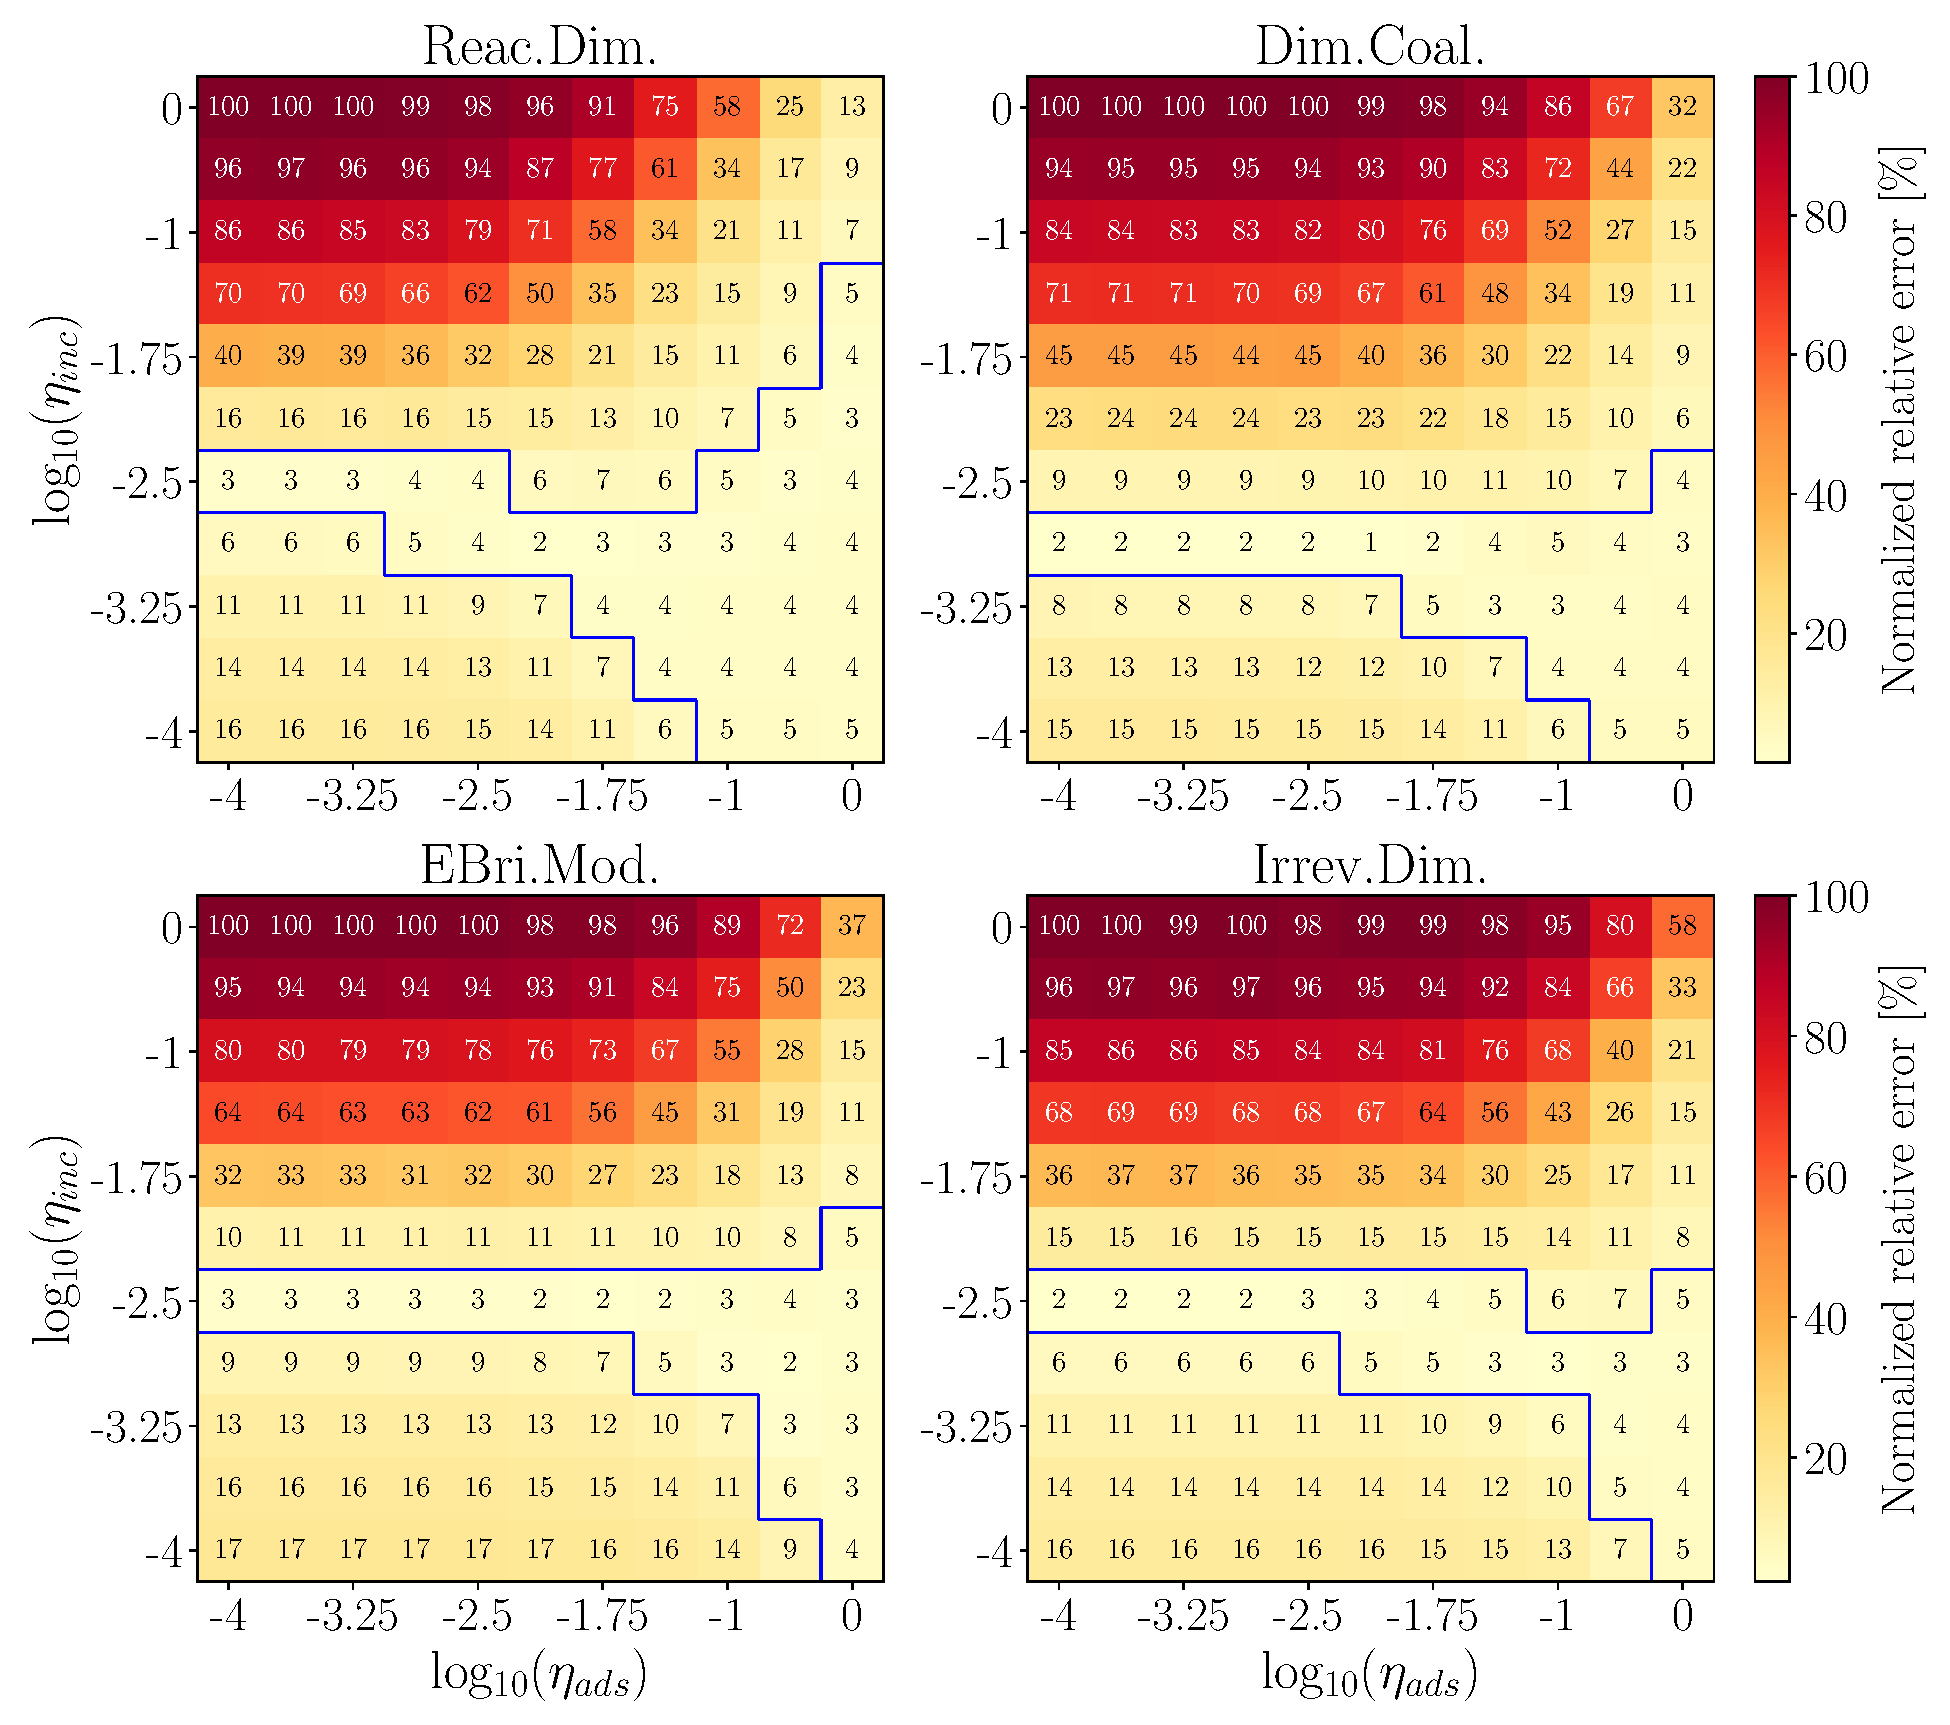
\includegraphics[width=0.8\textwidth]{Figures/Results/Shocktube/Agafonov2016_cpr/5CH4_norm_yield_error_all.pdf}
	\caption{The relative error of CY normalized by the maximum value at $t=$1.5 ms for 5\%~$\mathrm{CH_4}$ obtained using Caltech mechanism and different inception models.}
	\label{fig:shockagof_yielderror_cpr} 
\end{figure}


%The model was run without soot (only the gas phase is simulated and no soot conversion allowed) to provide insight into the effect of temperature on the species involved in soot formation.

Figure~\ref{fig:SPC_cmf_cpr}a shows the CMF of soot precursors (individual PAHs and total) and $\mathrm{C_2H_2}$ at 1.5 ms across the studied temperature range, with the soot model deactivated. While PAH precursors exhibit a bell-shaped profile, the CMF of $\mathrm{C_2H_2}$ increases linearly with temperature and plateaus near 85\% at $\mathrm{T_5} \approx 2400$ K. Among the considered PAHs, A2, A2R5, and A4R5 account for most of the carbon and are likely major contributors to soot inception and surface growth. The significant variation in PAH CMF highlights the impact of precursor selection on inception flux, surface growth rates, and their temperature sensitivity. Figure~\ref{fig:shockagof_yieldspc_cpr} illustrates the effect of excluding five-membered ring PAHs (A2R5, A3R5, and A4R5) from the soot precursors on the CY and $d_p$. As expected, excluding these species leads to a substantial reduction in CY: a factor of 3 for Reactive Dimerization and a factor of 12 for E-Bridge Modified model. The peak CY temperature remains nearly unchanged for E-Bridge Modified model but shifts to 2100 K for other inception models. The impact on $d_p$ is less pronounced, showing a decrease for Reactive Dimerization and a slight increase for other models in the $2100-2500$ K range.

\begin{figure}[H]
	\centering
	\begin{subfigure}[t]{0.4\textwidth}
		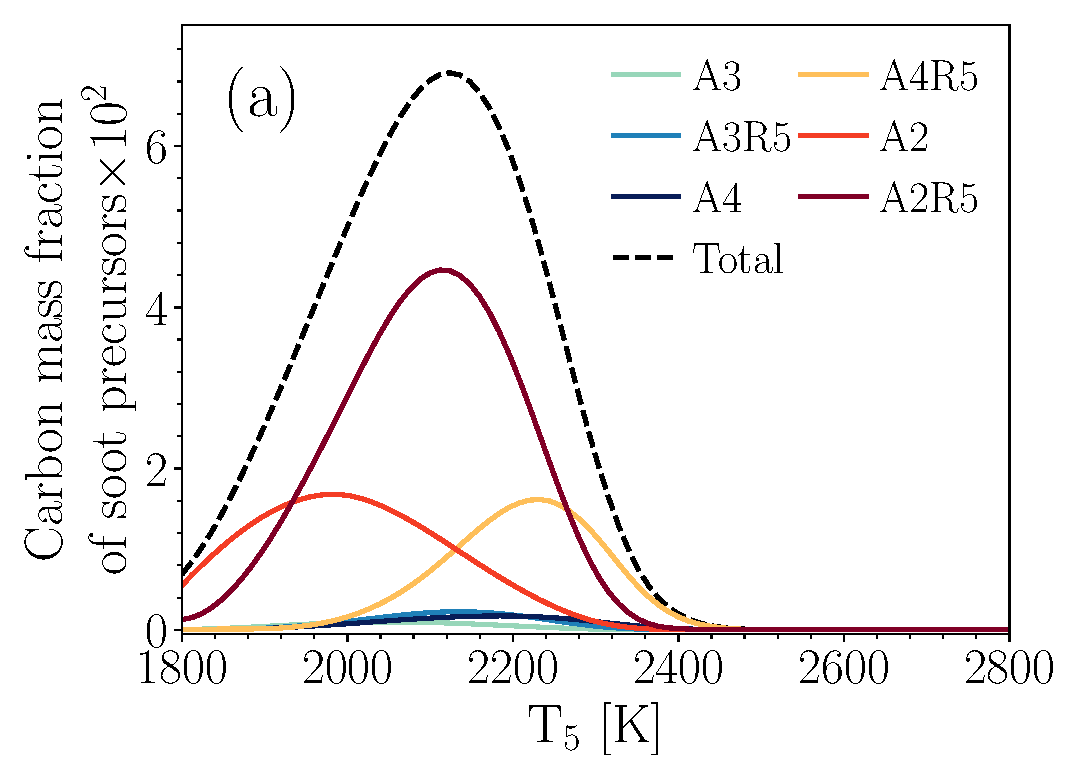
\includegraphics[width=1\textwidth]{Figures/Results/Shocktube/Agafonov2016_cpr/SPC_cmf_separate.pdf}
	\end{subfigure}
	\begin{subfigure}[t]{0.36\textwidth}
		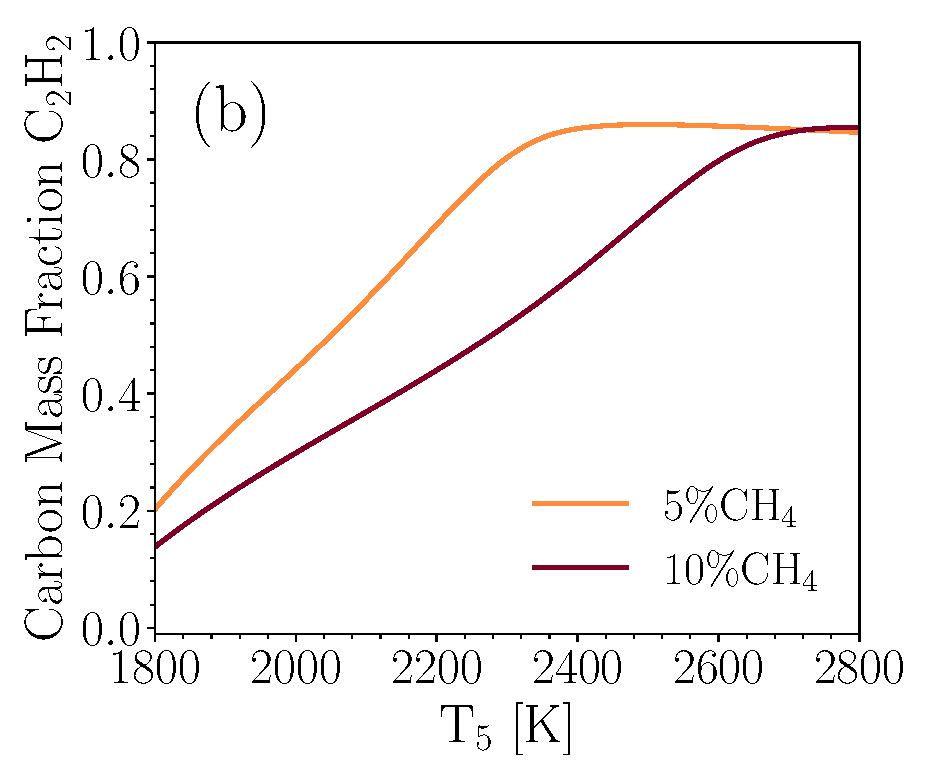
\includegraphics[width=1\textwidth]{Figures/Results/Shocktube/Agafonov2016_cpr/C2H2_cmf.pdf}
	\end{subfigure}
	\caption{The bell-shape temperature profile of carbon mass fraction of soot precursors (A2 and larger) combined (a) and $\mathrm{C_2H_2}$ (b) at $t=$1.5 ms during pyrolysis of 5\% (red line) and 10\%~$\mathrm{CH_4}$-Ar (green line) obtained using CPR model with Caltech mechanism without considering soot.}
	\label{fig:SPC_cmf_cpr} 
\end{figure}





Next set of simulations were conducted by using equal adjustment factors ($\eta_{inc}=\eta_{ads}$) to minimize the prediction error of CY. Figure~\ref{fig:shockagof_yield_dp_cpr} compares CY and $d_p$ from various inception models with experimental extinction data~\citep{agafonov2016unified}. A skew exponential curve (black dotted line) was fitted to highlight the CY trend and its peak near 12\%. Soot CY follows a bell-shaped profile similar to that of soot precursors, as inception flux and mass growth directly depend on precursor concentrations. Reactive Dimerization predicts higher CY at lower temperatures, while E-Bridge Modified model shifts the peak to higher temperatures due to a different temperature dependency—primarily governed by PAH dehydrogenation via an Arrhenius rate law, in contrast to physical PAH collisions in other models. The predicted $d_p$ increases with $\mathrm{T_5}$, reaching a maximum of 12.5 nm at 2700 K, where yield is minimal ($\approx 10^{-7}$), and then drops to the model's minimum allowed value of 2 nm. Figure~\ref{fig:shockagof_Nagg_np_cpr}a shows that $N_{pri}$ peaks at $\approx 2200$ K, aligning with the peak in CY. This is expected since $N_{pri}$ depends solely on the inception flux, which is highest when PAH concentrations peak. Increased coagulation rates reduce $N_{agg}$ in the $2000-2500$ K range.% The coagulation characteristic time depends on $N_{agg}$ and $\beta$, which is temperature dependent. 
Reactive Dimerization model yields the fewest particles ($N_{pri}$ and $N_{agg}$) because more precursors are directed toward surface growth. Consequently, $n_p$ is lowest for Reactive Dimerization model. Differences between inception models are more evident in $n_p$ than in $d_p$, influencing predicted particle morphology. These differences become more pronounced at longer residence times. For instance, Dimer Coalescence model predicts a more ramified agglomerate ($n_p = 38$) compared to Reactive Dimerization model ($n_p = 12$). Additional morphological data could help constrain inception and surface growth rates in soot models.

\begin{figure}[H]
	\centering
	\begin{tikzpicture}
		\draw (0, 0) node[inner sep=0] 	{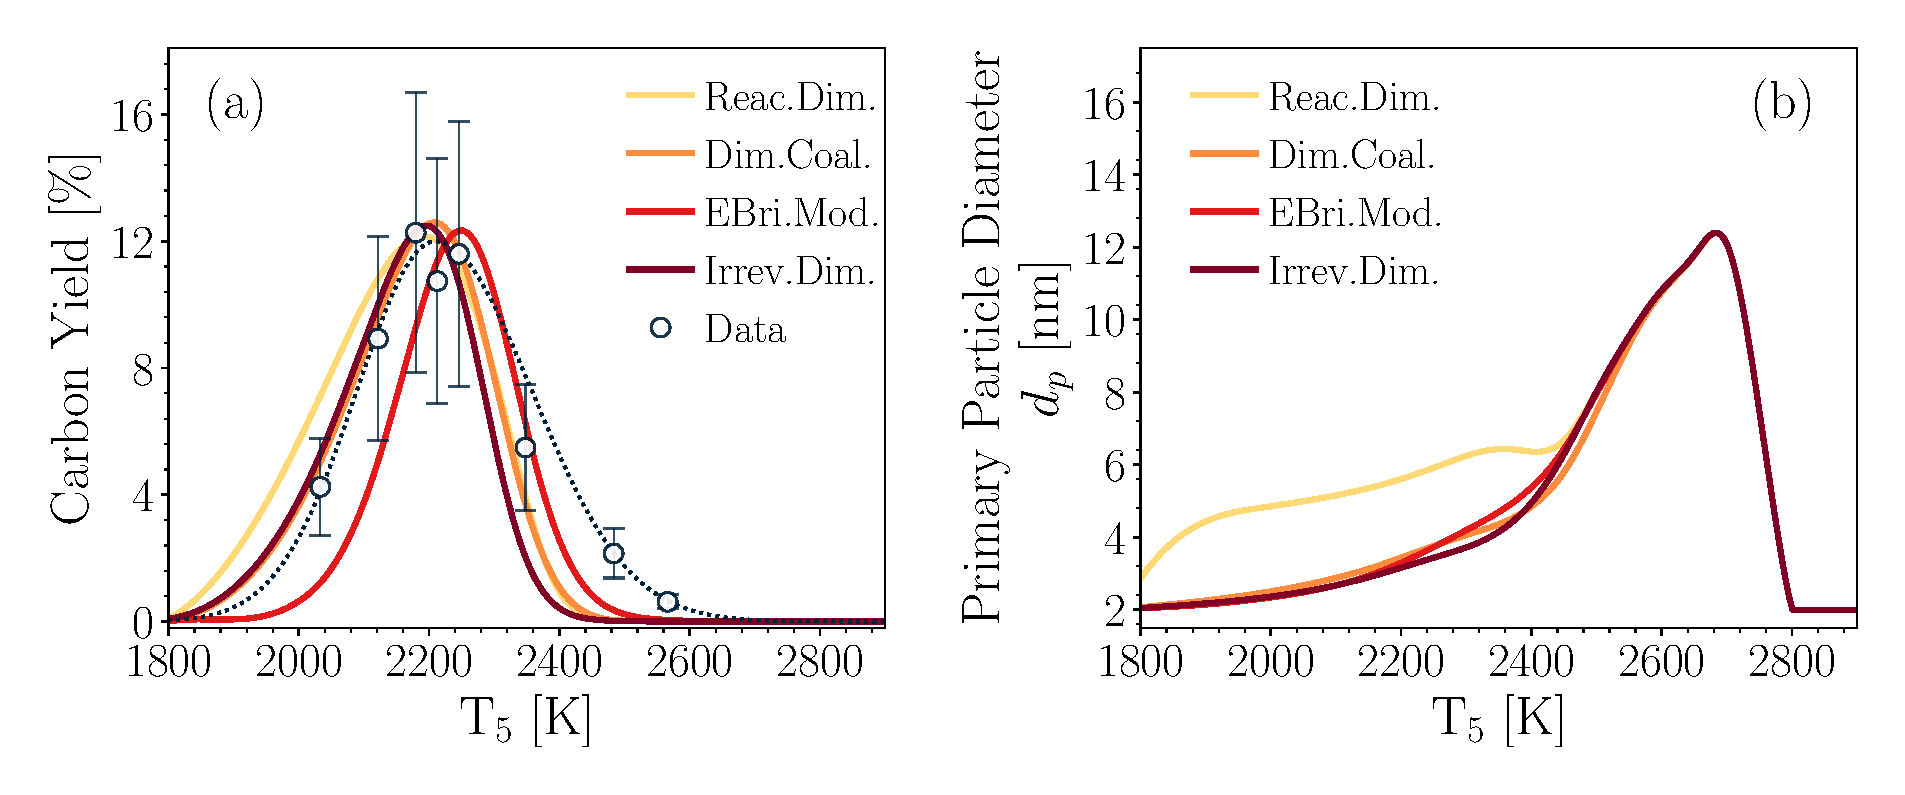
\includegraphics[width=0.8\textwidth]{Figures/Results/Shocktube/Agafonov2016_cpr/carbon_yield_d_p_5CH4.pdf}};
		\draw (-0.85, 0.42) node {\scriptsize{\cite{agafonov2016unified}}};
		%\draw (2.42, -0.23) node {\scriptsize{\cite{agafonov2016unified}}};
	\end{tikzpicture}
	\caption{The bell-shape temperature profile of CY at $t=$1.5 ms (a) and increasing primary particle diameter, $d_p$, obtained using Caltech mechanism and different inception models optimized using equal adjustment factors to minimize the prediction with extinction measurements~\citep{agafonov2016unified}. The dashed line was added to show the trend in the measurements.}
	\label{fig:shockagof_yield_dp_cpr} 
\end{figure}


\begin{figure}[H]
	\centering
	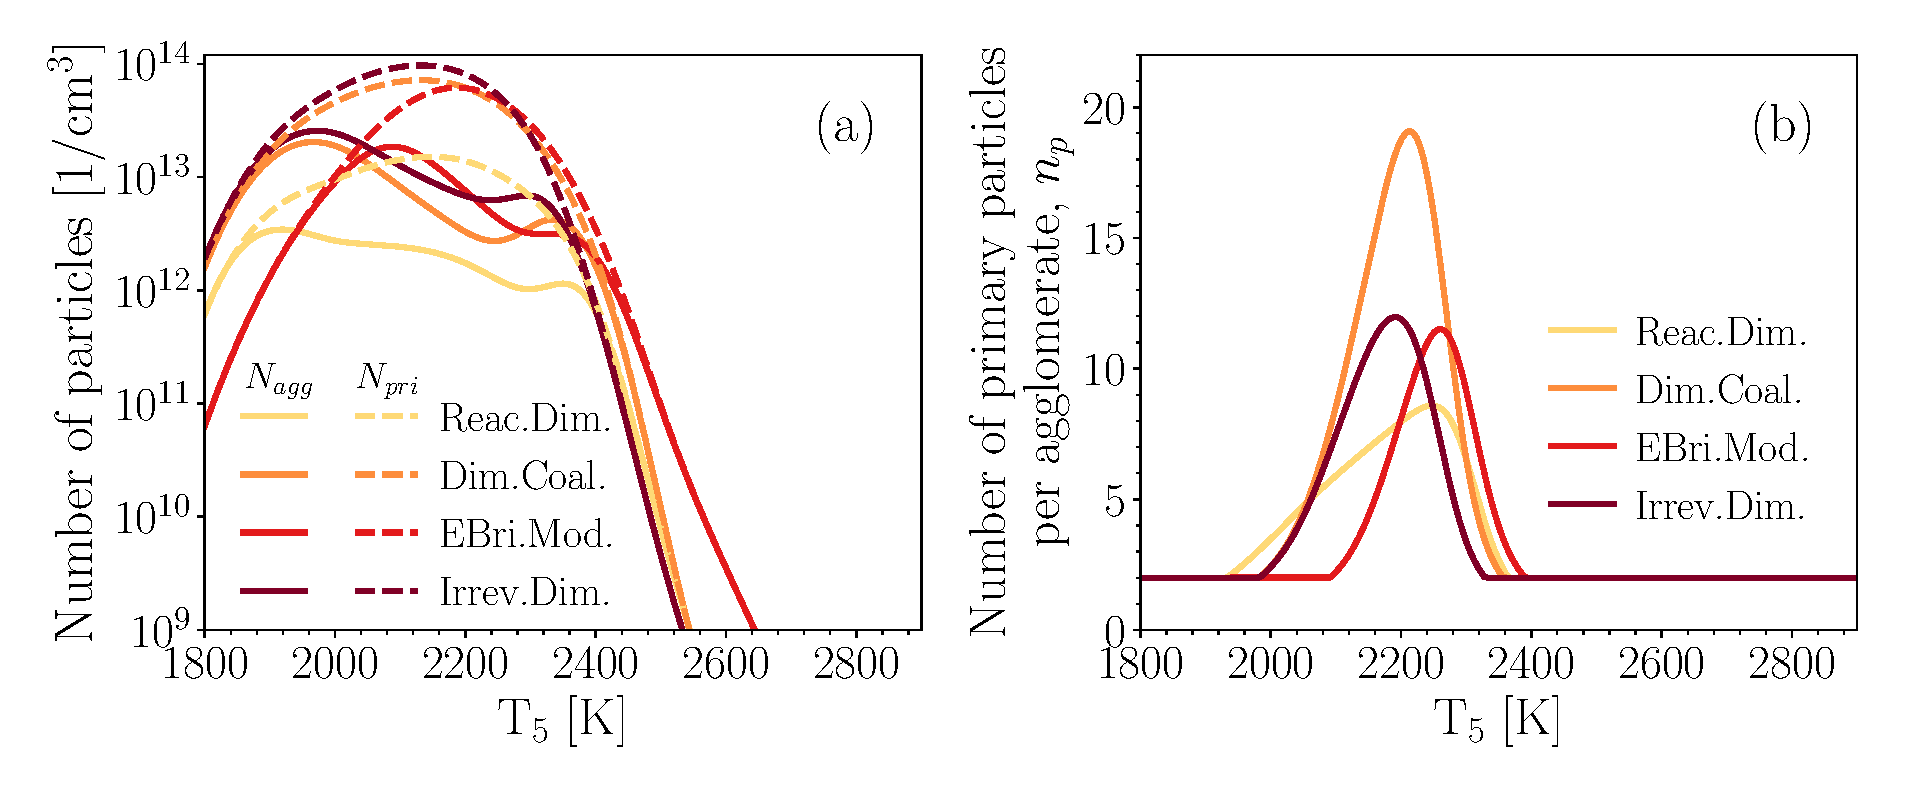
\includegraphics[width=0.8\textwidth]{Figures/Results/Shocktube/Agafonov2016_cpr/N_agg_n_p_5CH4.pdf}
	\caption{The temperature dependence of total number of agglomerates, $N_{agg}$ (a), number of primary particles per agglomerate, $n_p$ (b) at $t=$1.5 ms obtained using Caltech mechanism and different inception models optimized using equal adjustment factors to minimize the prediction with extinction measurements~\citep{agafonov2016unified}.}
	\label{fig:shockagof_Nagg_np_cpr} 
\end{figure}

The differences between inception models in prediction of $d_p$  is overall negligible except for Reactive Dimerization model, which predicts a larger $d_p$ in $\mathrm{T_5}<2500$. The $d_p$ trends can be better understood by examining Equation~\eqref{eqn:d_p} indicating that $d_p$ is proportional of the third-root of $C_{tot}/N_{pri}$. $C_{tot}$ describes total carbon mass converted to soot through inception and surface growth while $N_{pri}$ is only determined by inception flux. As a result, $d_p$ is controlled by the ratio of surface growth (HACA and PAH adsorption) rate to inception flux. The ratio of carbon mass gained up to 1.5 ms by each pathway to the total soot carbon mass is calculated and shown in Figure~\ref{fig:shockagof_carbon_map_cpr}. PAH adsorption is the dominant soot mass growth pathway for Reactive Dimerization model in $\mathrm{T_5}<2000$ K (Figure~\ref{fig:shockagof_carbon_map_cpr}a) that results in larger $C_{tot}/N_{pri}$ and $d_p$ values, but inception is dominant for the other inception models. The CMF of inception decreases with temperature for all inception models leading to higher $d_p$ values up to 2700 K and it increases afterwards that changes $d_p$ trends.


\begin{figure}[H]
	\centering
	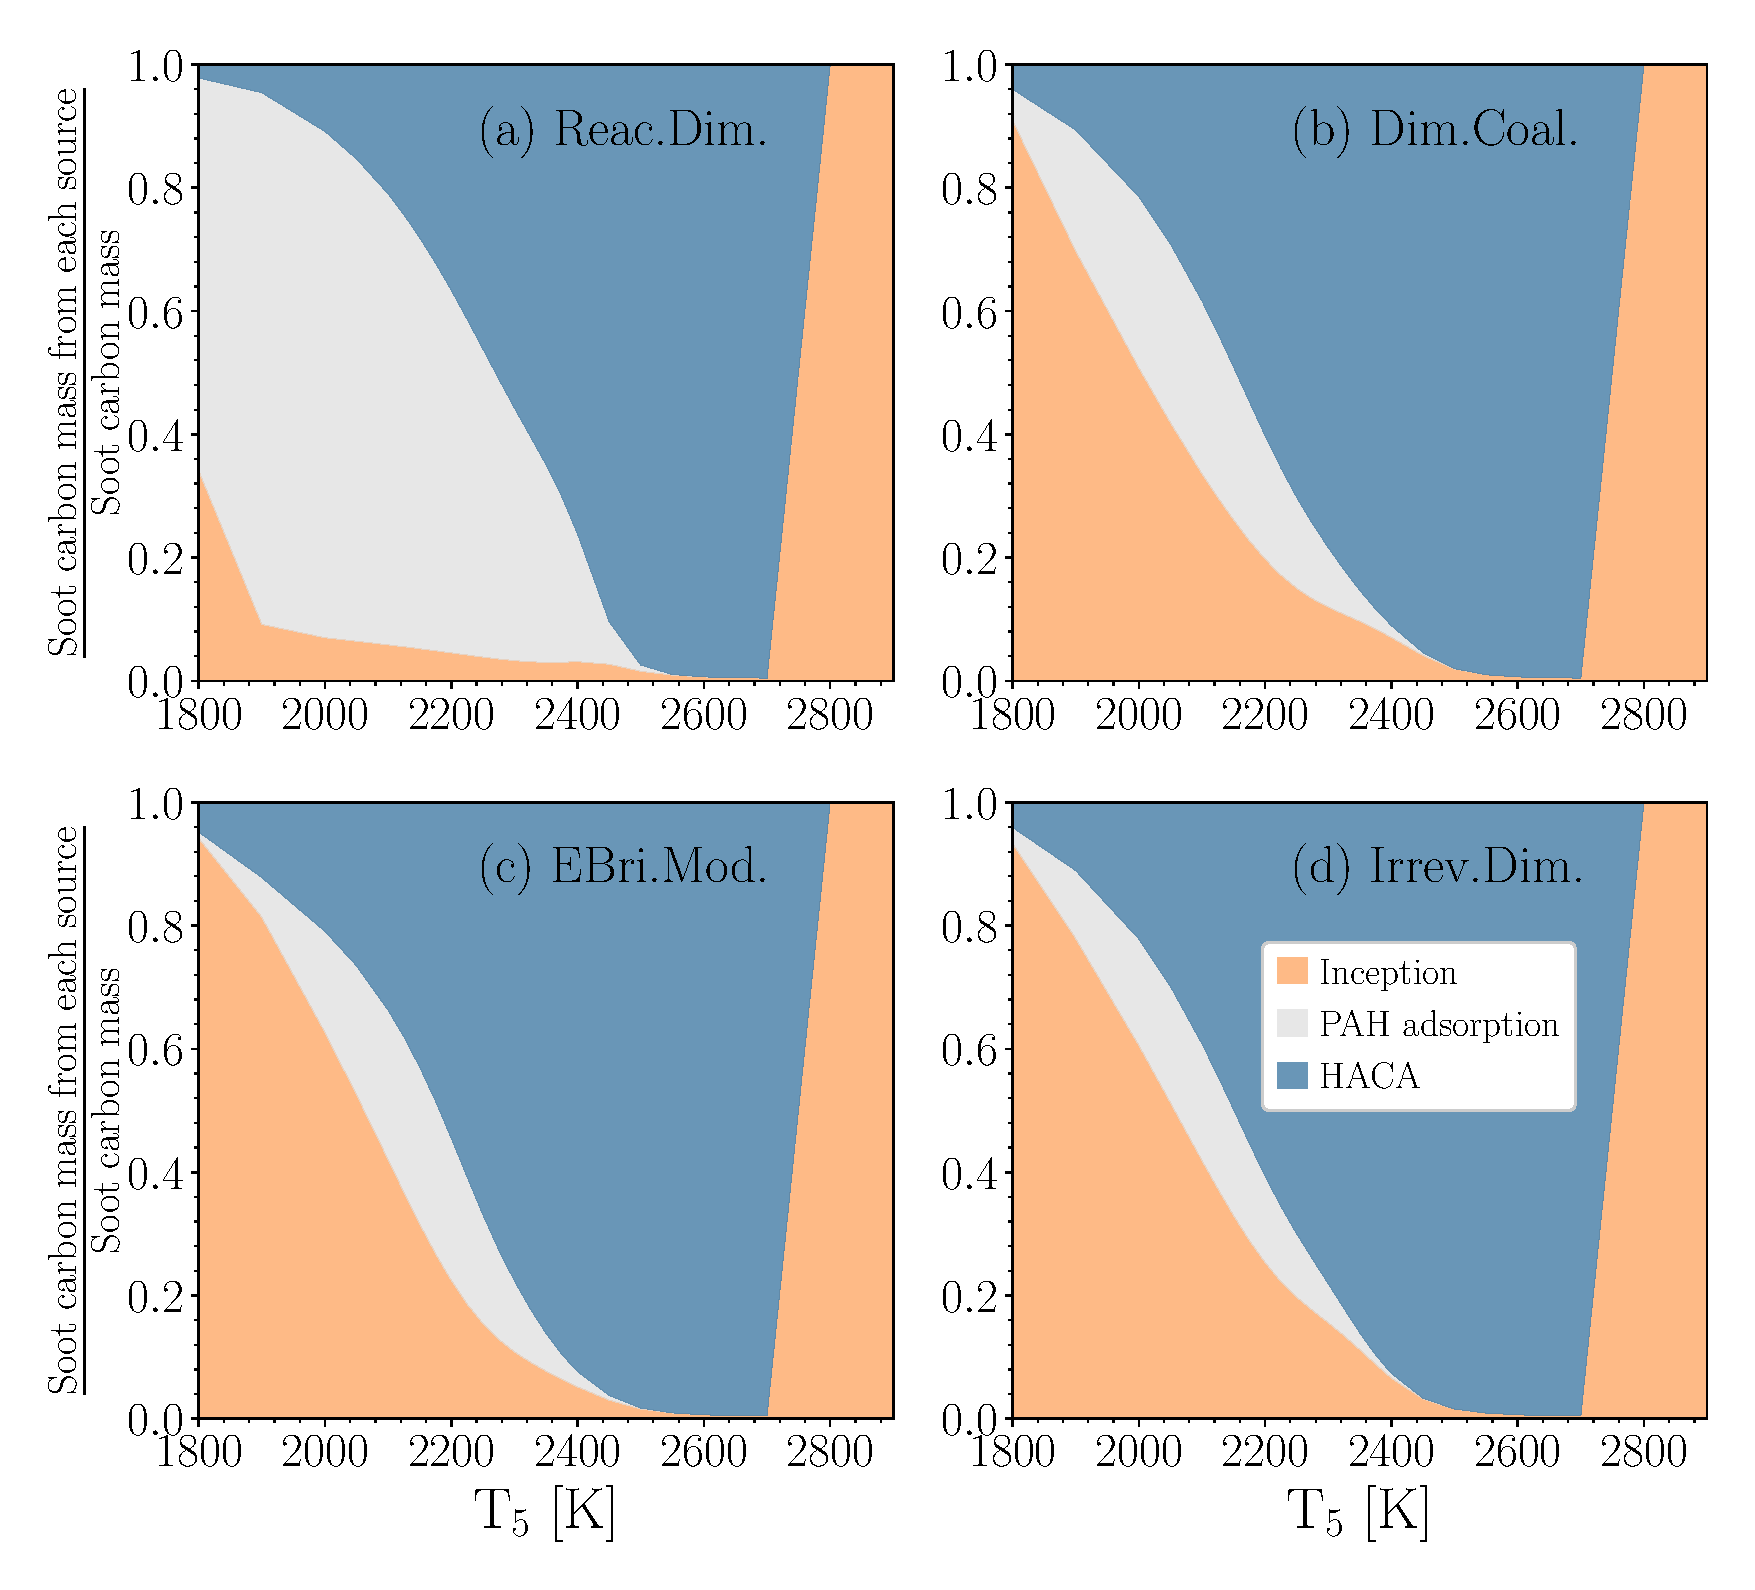
\includegraphics[width=0.8\textwidth]{Figures/Results/Shocktube/Agafonov2016_cpr/C_tot_distmap_5CH4.pdf}
	\caption{The soot carbon mass from inception, PAH adsorption and HACA normalized by total soot carbon mass at $t=$1.5 ms for 5\% in Ar obtained using Caltech mechanism and different inception models calibrated to minimize the prediction with extinction measurements~\citep{agafonov2016unified}.}
	\label{fig:shockagof_carbon_map_cpr} 
\end{figure}

Figure~\ref{fig:shockagof_yield_maxincads_cpr} shows that optimizing models with minimum $\eta_{inc}$ and $\eta_{ads}$ yields similar CY predictions across inception models, except E-Bridge Modified model, which shifts slightly toward higher temperatures. The minimum adsorption case has a higher peak and narrower profile compared to the minimum inception case. Figure~\ref{fig:shockagof_dp_maxincads_cpr} demonstrates the variation in $d_p$ among the inception models with the minimum inception (solid line) mode compared to the minimum adsorption (dashed line) that show negligible sensitivity to the inception model. In the minimum inception mode, the majority of soot mass comes from PAHs, so $d_p$ shows a bell-shape profile with a peak close to the temperature of the peak CMF of precursors (dashed line in Figure~\ref{fig:SPC_cmf_cpr}). Reactive Dimerization model has the largest variation at the peak from 2 to 21 nm for the minimum inception and adsorption, respectively. The global adjustment factors were used to alter the contribution of precursors to inception and surface growth without changing the internal rate constants of inception models. A close agreement was achieved between the predicted and measured CY in different modes of inception and PAH adsorption that can result in different soot morphology. Characterizing primary particle size in the experiment can reduce the uncertainty in the model and restrict the range of expected inception and surface growth rate and highlight the need to account for missing pathways and phenomena involved in soot yield and morphology.

\begin{figure}[H]
	\centering
	\begin{tikzpicture}
			\draw (0, 0) node[inner sep=0] 	{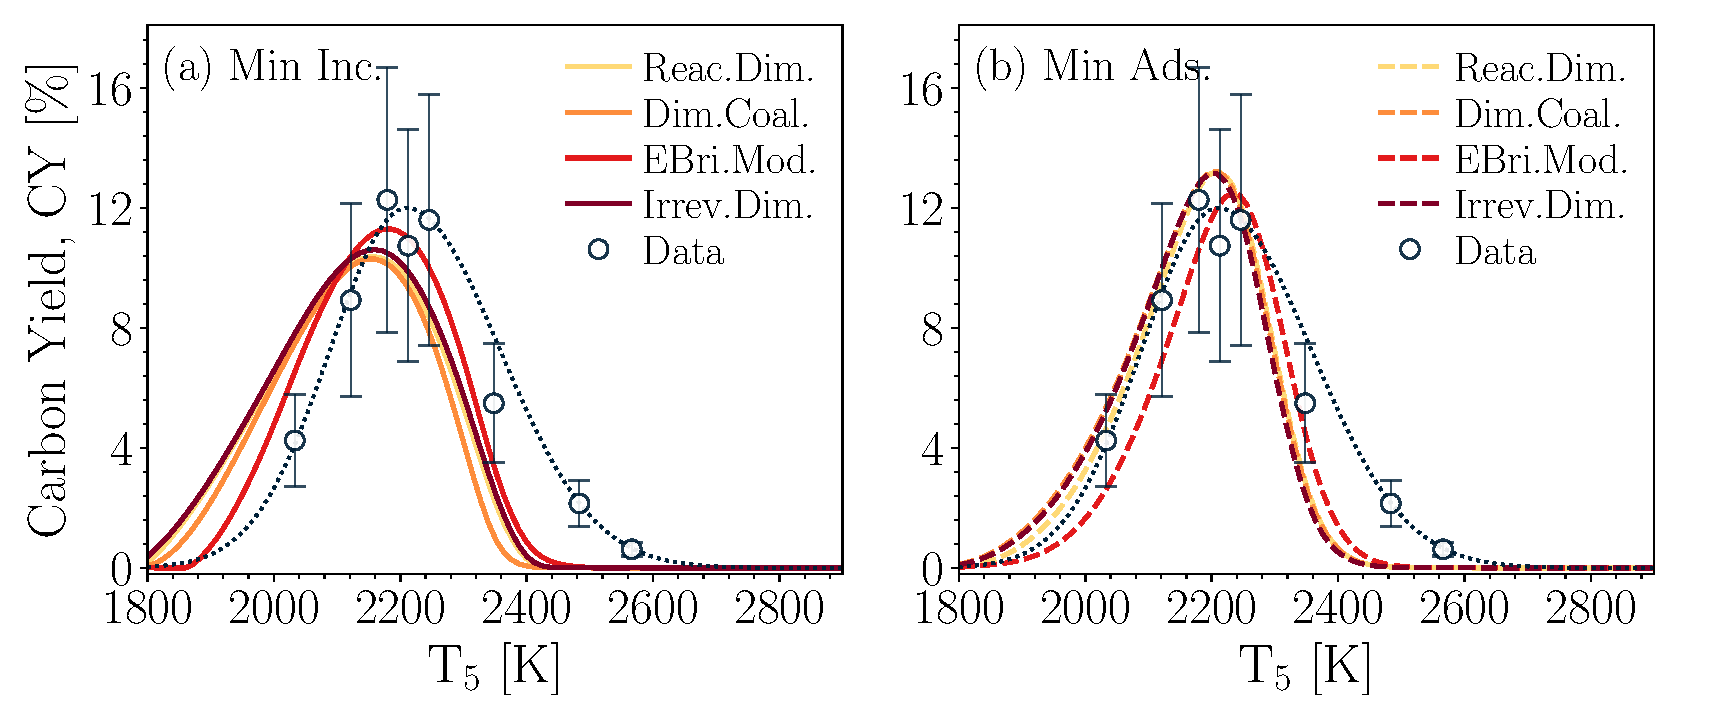
\includegraphics[width=0.8\textwidth]{Figures/Results/Shocktube/Agafonov2016_cpr/carbon_yield_maxincads_combined.pdf}};
			\draw (-0.48, 0.75) node {\scriptsize{\cite{agafonov2016unified}}};
			\draw (5.33, 0.75) node {\scriptsize{\cite{agafonov2016unified}}};
		\end{tikzpicture}
	\caption{The comparison of CY at $t=$1.5 ms when the minimum inception (a) and the minimum PAH adsorption (b) adjustment factors were applied to minimize the prediction error compared to measurements~\citep{agafonov2016unified} for 5\%~$\mathrm{CH_4}$-Ar obtained using Caltech mechanism and different inception models.}
	\label{fig:shockagof_yield_maxincads_cpr} 
\end{figure}

%\begin{figure}[H]
%	\centering
%	\begin{tikzpicture}
%		\draw (0, 0) node[inner sep=0] 	{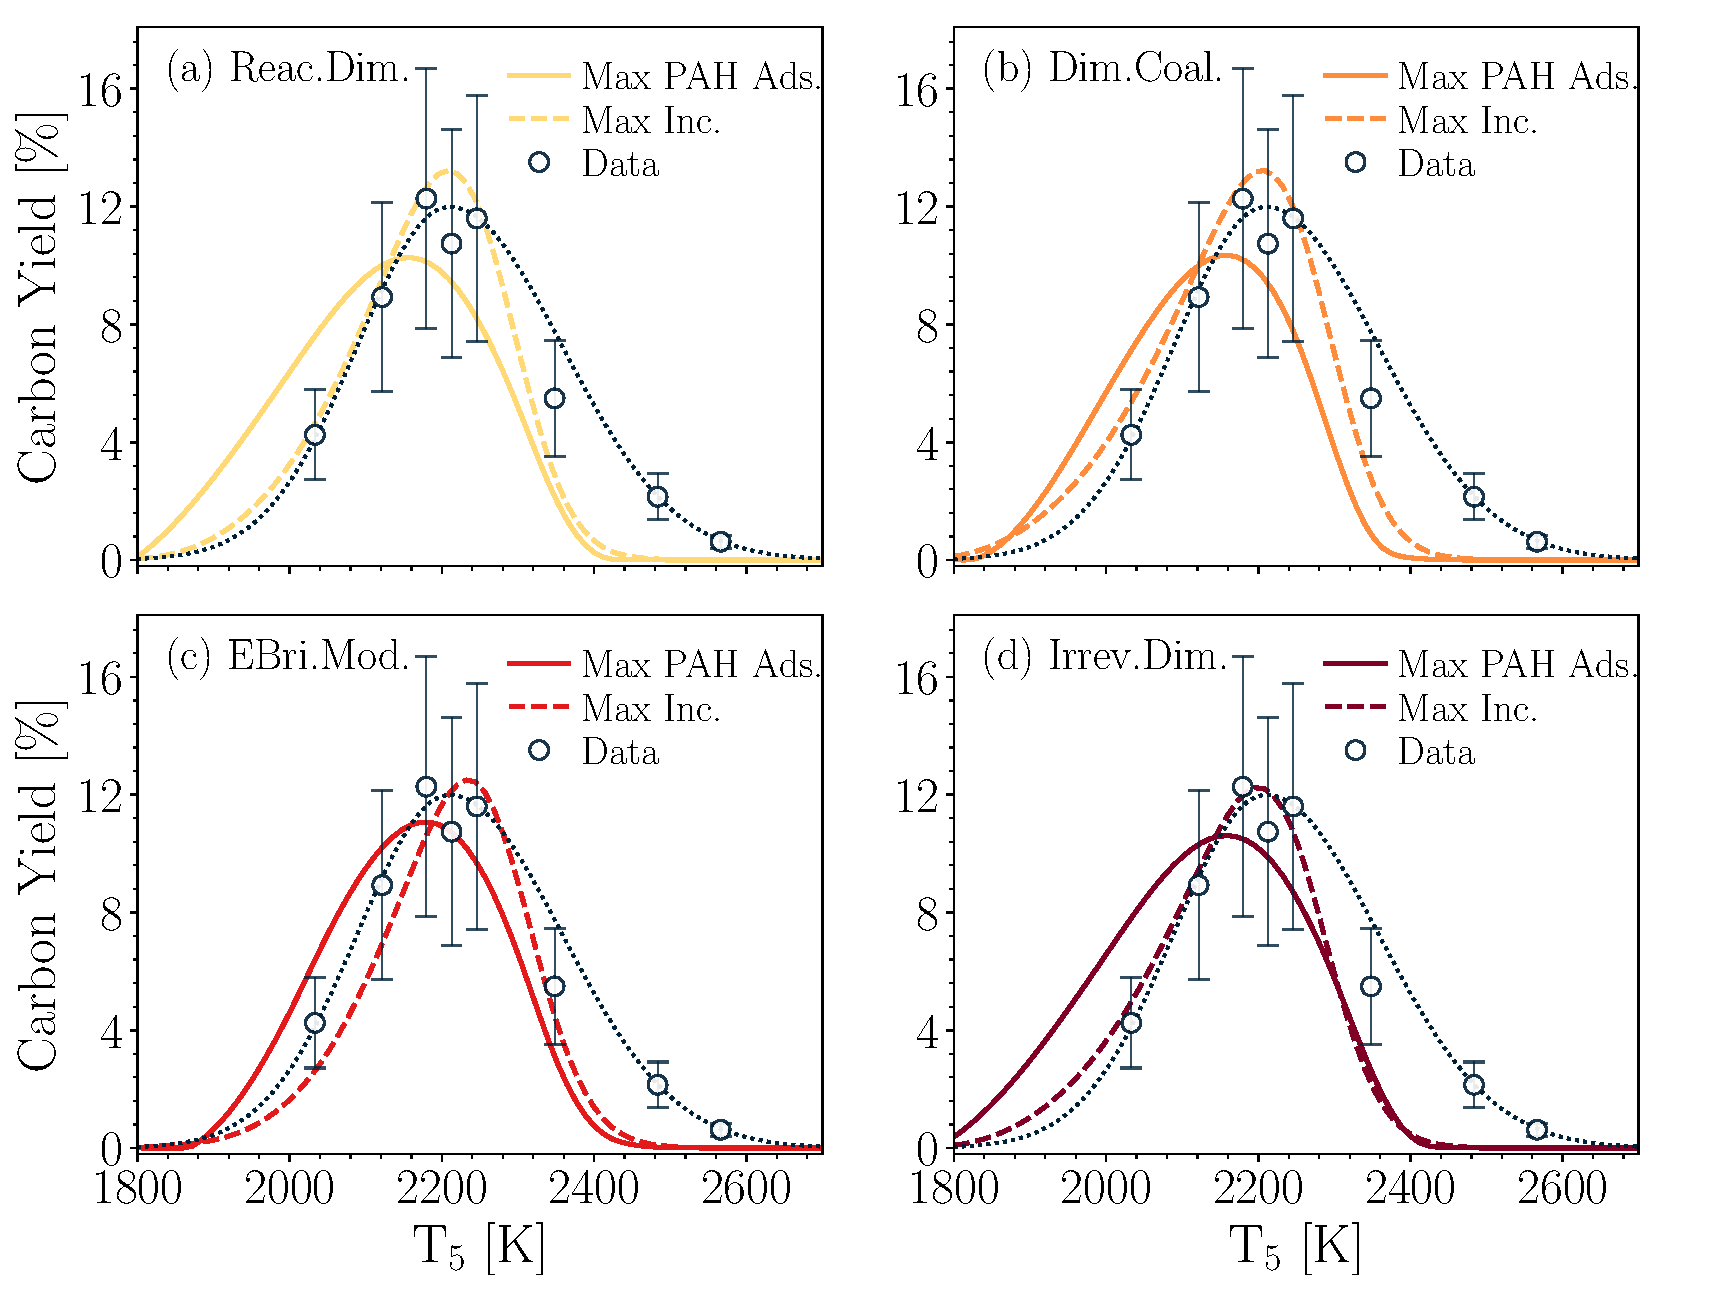
\includegraphics[width=0.8\textwidth]{Figures/Results/Shocktube/Agafonov2016_cpr/carbon_yield_maxincads.pdf}};
%		\draw (-0.48, -0.8) node {\scriptsize{\cite{agafonov2016unified}}};
%		\draw (5.33, -0.8) node {\scriptsize{\cite{agafonov2016unified}}};
%		\draw (-0.48, 3.36) node {\scriptsize{\cite{agafonov2016unified}}};
%		\draw (5.33, 3.36) node {\scriptsize{\cite{agafonov2016unified}}};
%	\end{tikzpicture}
%	\caption{The comparison of soot carbon yield at t=1.5 ms when maximum inception (dashed line) and PAH adsorption (solid line) were applied to minimized the prediction error compared to measurements~\citep{agafonov2016unified} for 5\% (a) and 10\%~$\mathrm{CH_4}$ (b) in Ar obtained using Caltech mechanism and different inception models.}
%	\label{fig:shockagof_yield_maxincads_cpr} 
%\end{figure}

\begin{figure}[H]
	\centering
	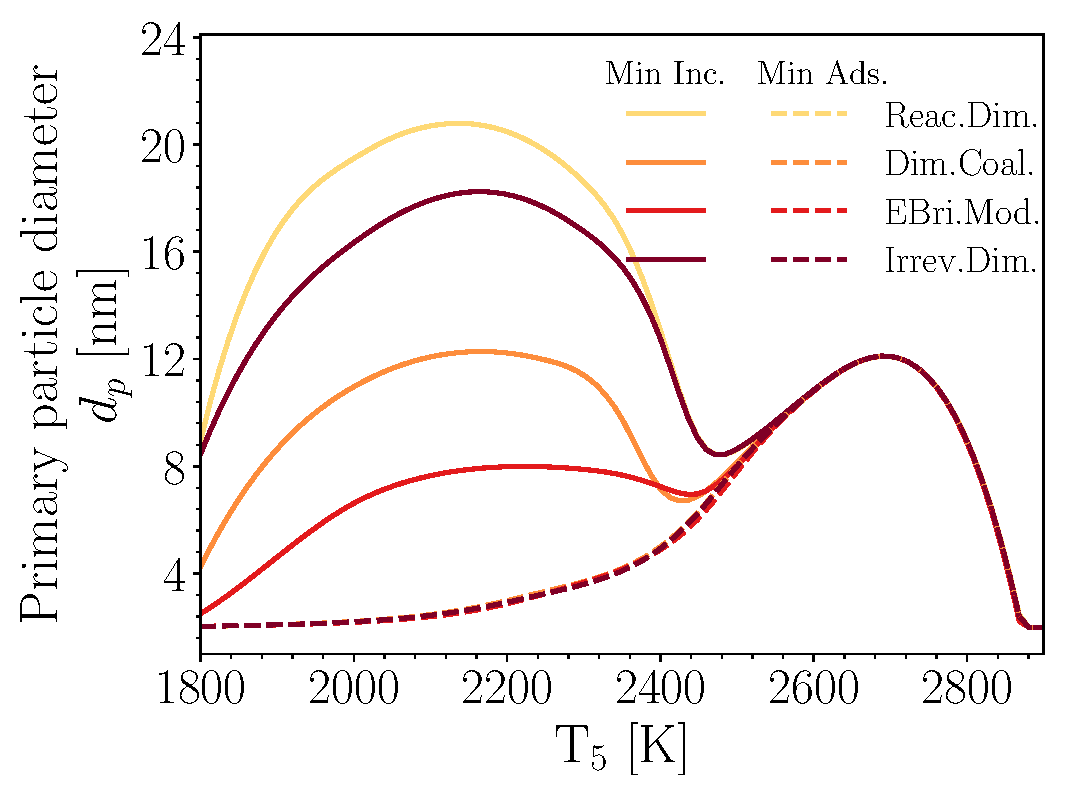
\includegraphics[width=0.5\textwidth]{Figures/Results/Shocktube/Agafonov2016_cpr/d_p_maxincads_combined.pdf}
	\caption{The comparison of mean primary particle, $d_p$, at $t=$1.5 ms when the minimum inception (solid lines) and adsorption (dashed lines) were applied to minimized the prediction error compared to measurements~\citep{agafonov2016unified} for 5\%-Ar obtained using Caltech mechanism and different inception models.}
	\label{fig:shockagof_dp_maxincads_cpr} 
\end{figure}

%\begin{figure}[H]
%	\centering
%	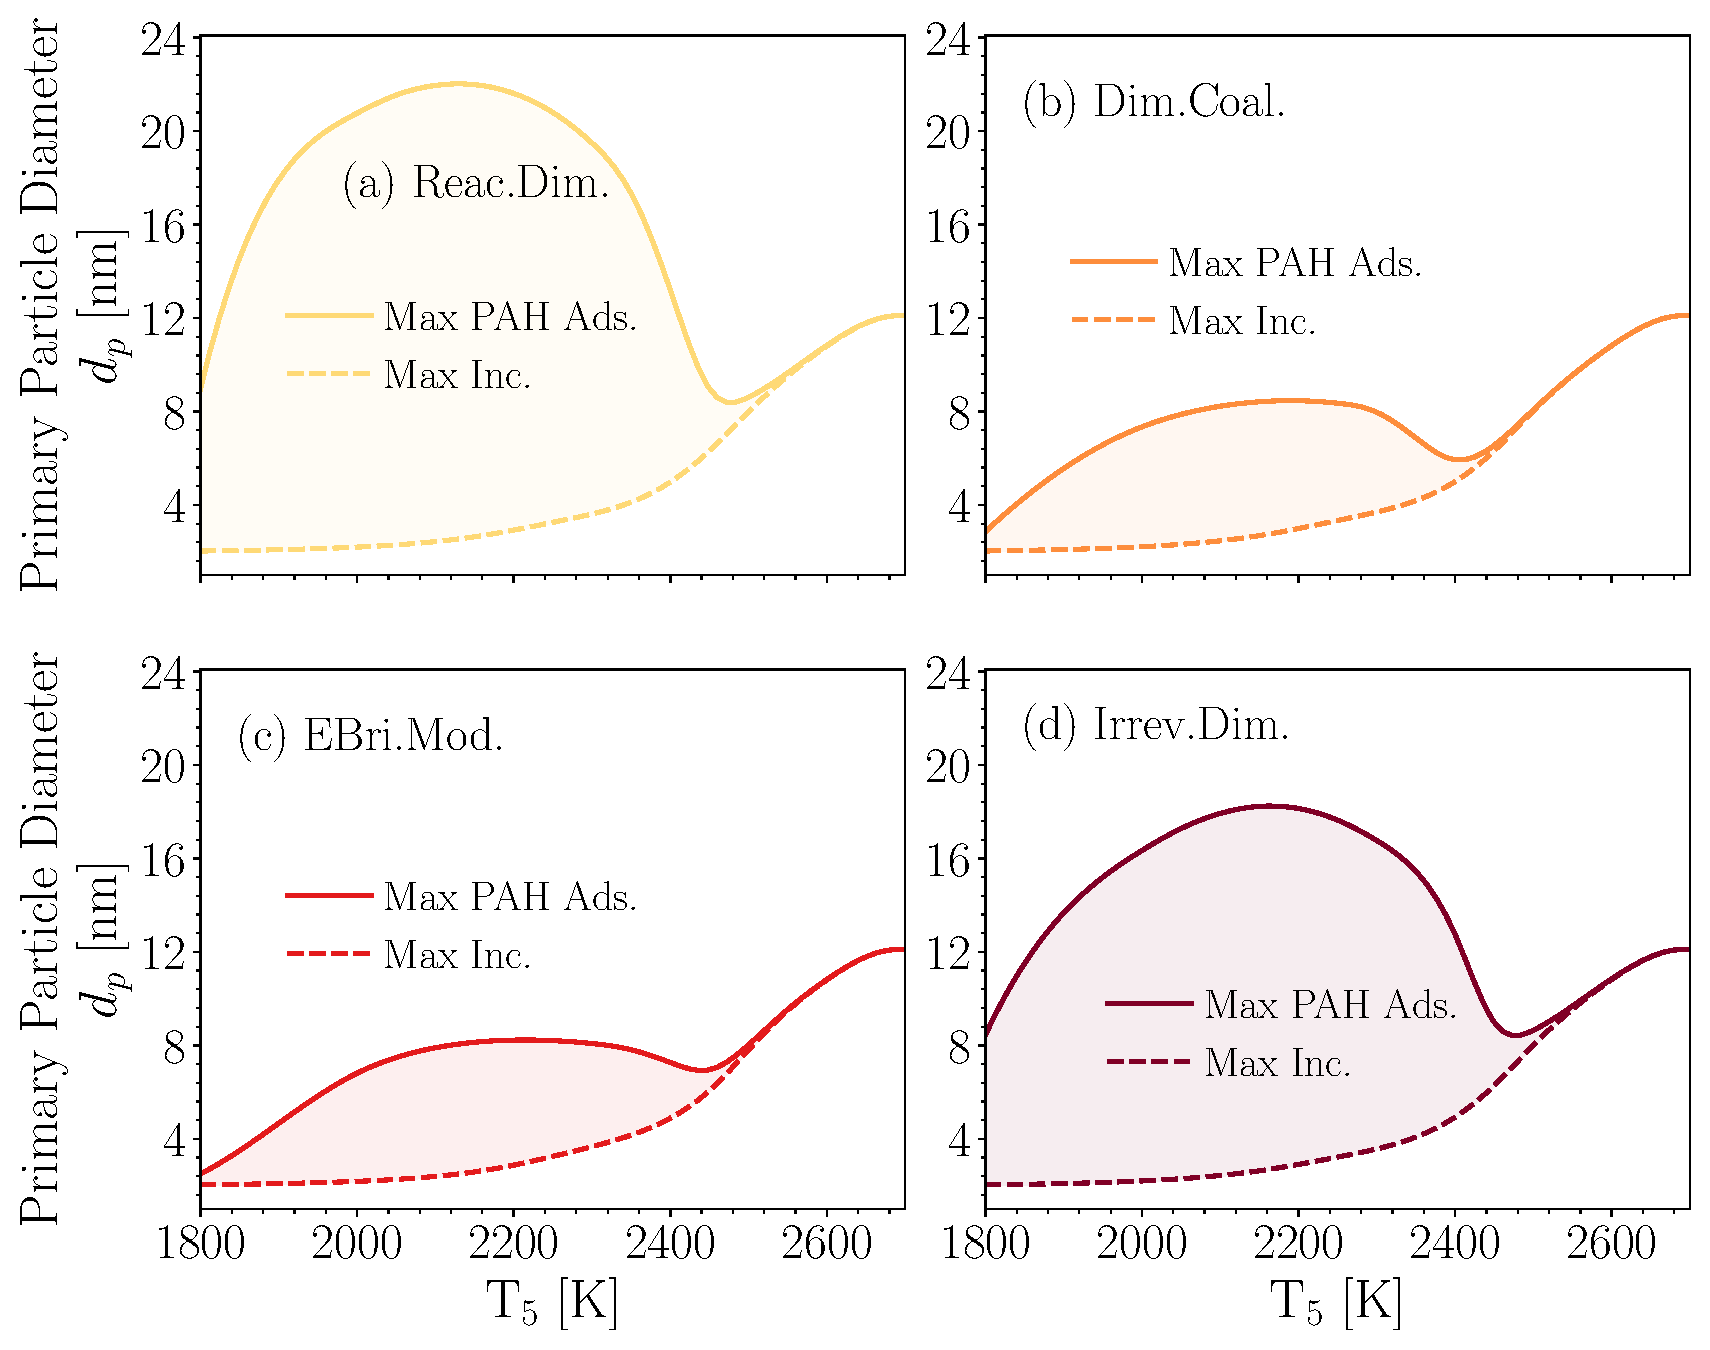
\includegraphics[width=0.8\textwidth]{Figures/Results/Shocktube/Agafonov2016_cpr/d_p_maxincads.pdf}
%	\caption{The comparison of mean primary particle, $d_p$ at t=1.5 ms when maximum inception and PAH adsorption were applied to minimized the prediction  error compared to measurements~\citep{agafonov2016unified} for 5\% (a) and 10\%~$\mathrm{CH_4}$ (b) in Ar obtained using Caltech mechanism and different inception models.}
%	\label{fig:shockagof_dp_maxincads_cpr} 
%\end{figure}

%\subsection{Methane pyrolysis in shock-tube using constant volume reactor}

%The pyrolysis of 5\% and 10\% $\mathrm{CH_4}$-Ar was investigated using a constant volume reactor model (CVR) for the post-shock temperature, $T_5$ range of 1800-3000 K, and pressure, $P_5$ range of 4.7-7.1 bar. $P_5$ was assumed to linearly increase with $T_5$ across the simulation cases. Caltech mechanism was used and the inception models were calibrated in order to match carbon yield at t=1.5 ms with the measurement~\citep{agafonov2016unified} using a dual-beam absorption–emission technique. \citet{agafonov2016unified} reported yield$\times$E(m) at $\mathrm{\lambda}$=632~nm, and yield data was retrieved using E(m)=0.37 suggested therein. 


%\begin{figure}[H]
%	\centering
%	\begin{subfigure}[t]{0.4\textwidth}
%		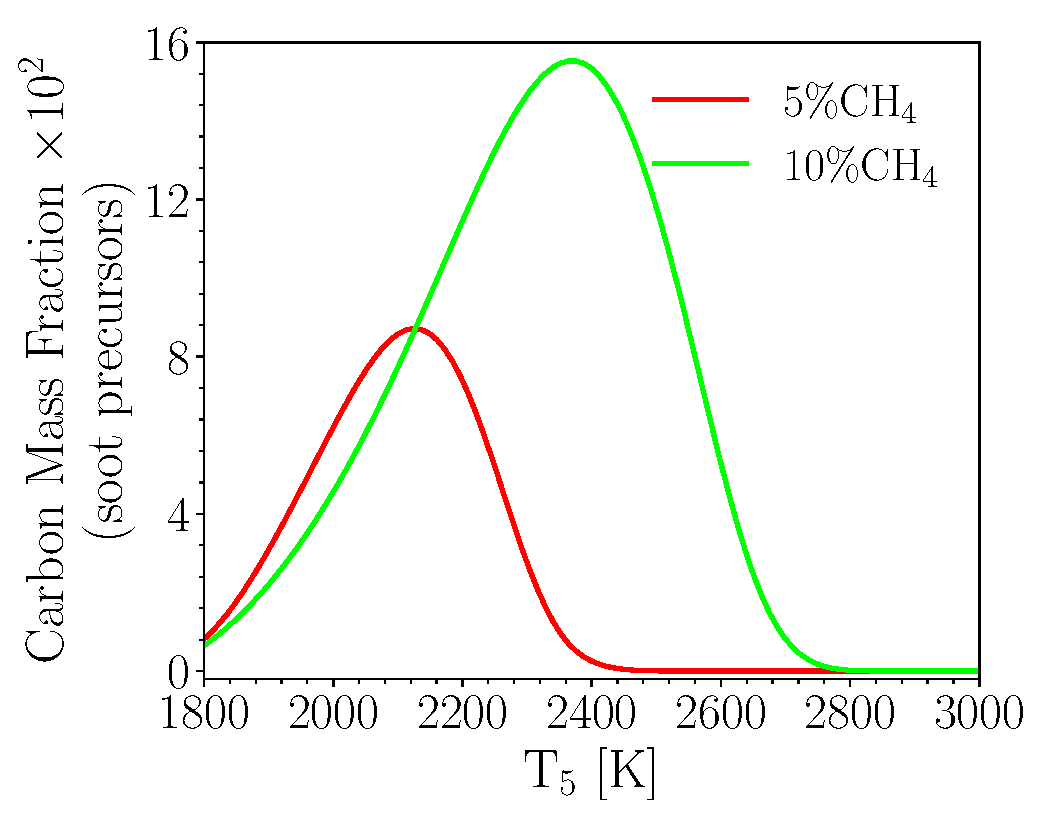
\includegraphics[width=1\textwidth]{Figures/Results/Shocktube/Agafonov2016_cvr/SPC_cmf.pdf}
%	\end{subfigure}
%	\begin{subfigure}[t]{0.4\textwidth}
%		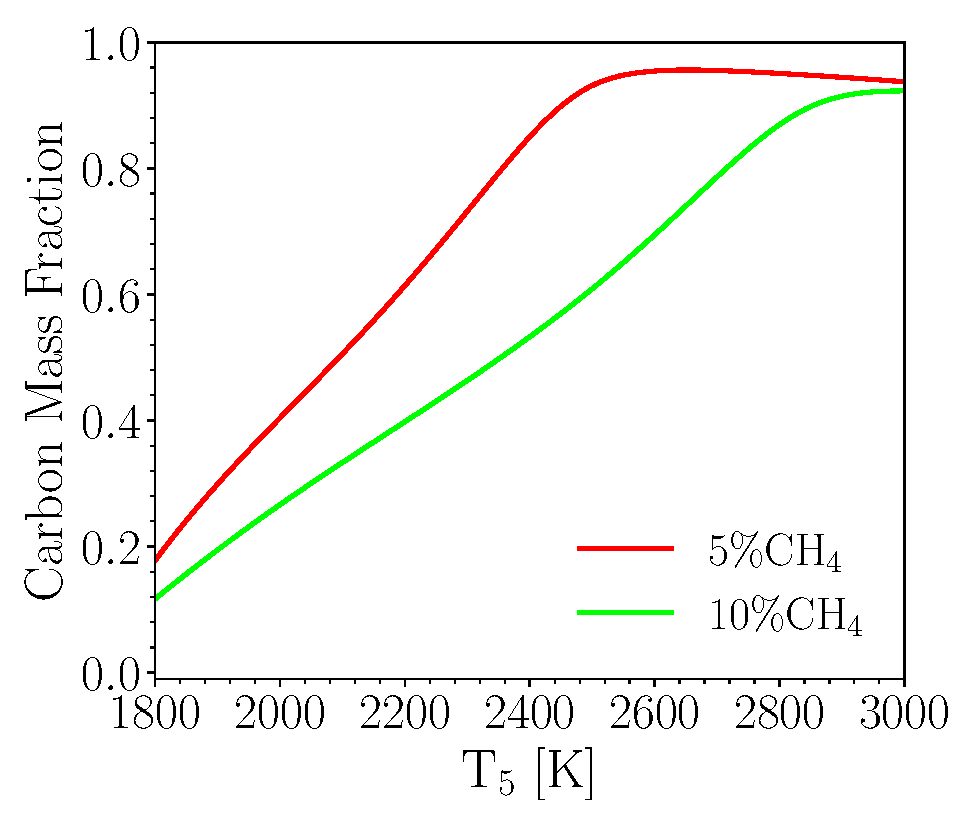
\includegraphics[width=1\textwidth]{Figures/Results/Shocktube/Agafonov2016_cvr/C2H2_cmf.pdf}
%	\end{subfigure}
%	\caption{The bell-shape temperature profile of carbon mass fraction of soot precursors (A2 and larger) combined (a) and $\mathrm{C_2H_2}$ (b) at t=1.5 ms during pyrolysis of 5\% (red line) and 10\%~$\mathrm{CH_4}$-Ar (green line) obtained using Caltech mechanism without considering soot}
%	\label{fig:SPC_cmf_cvr} 
%\end{figure}
%
%
%
%
%\begin{figure}[H]
%	\centering
%	\begin{tikzpicture}
%		\draw (0, 0) node[inner sep=0] 	{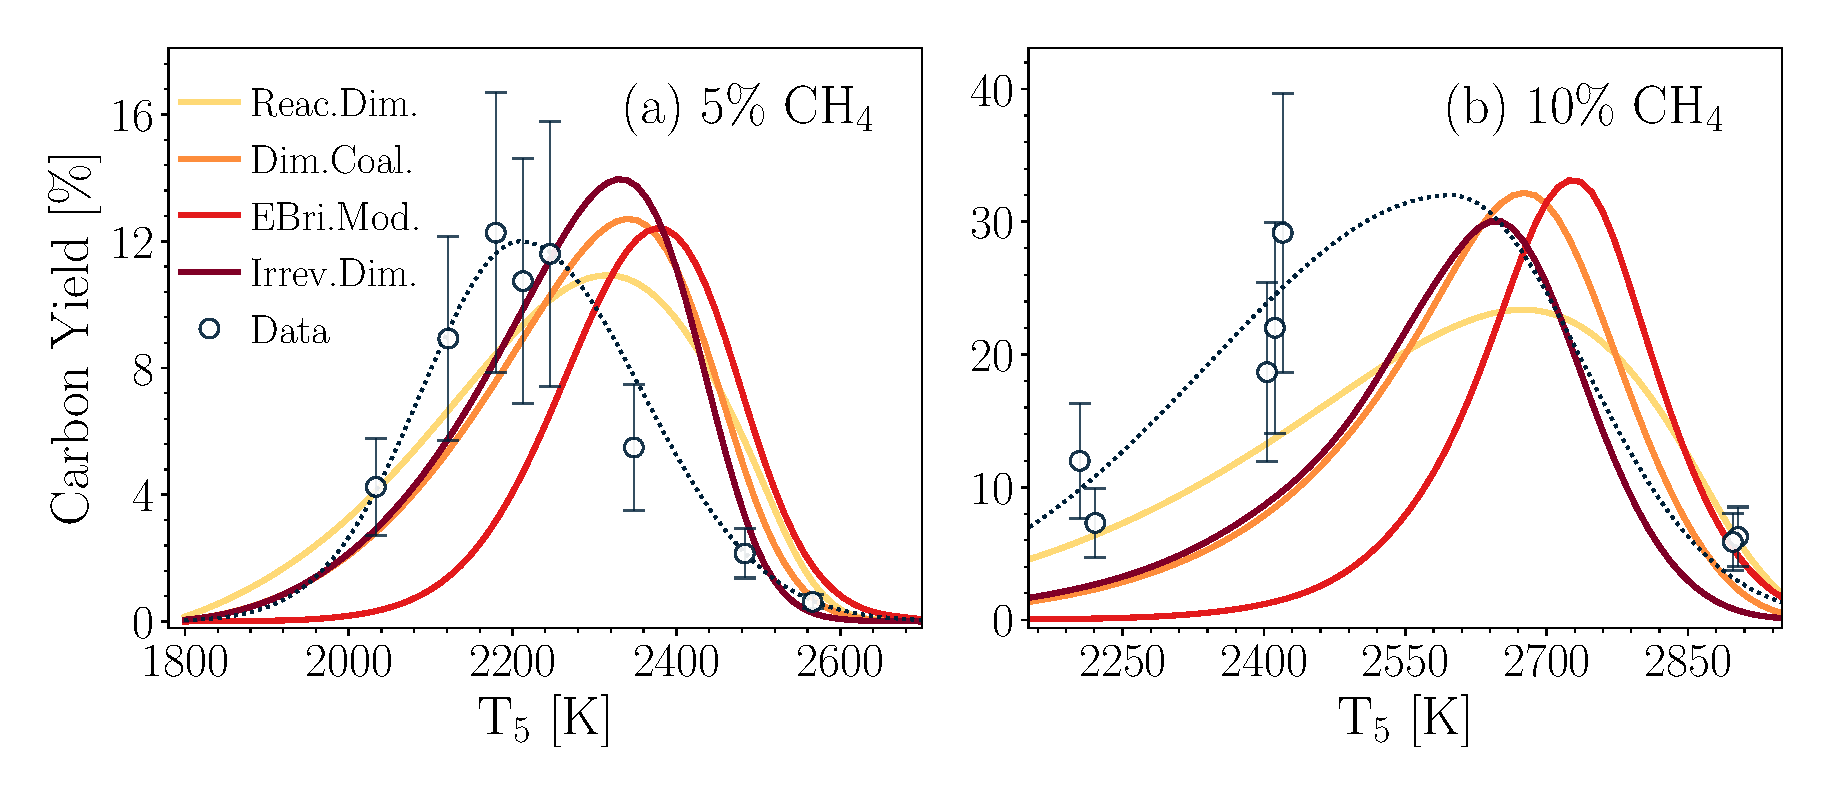
\includegraphics[width=0.8\textwidth]{Figures/Results/Shocktube/Agafonov2016_cvr/carbon_yield.pdf}};
%		\draw (-3.6, 0.42) node {\scriptsize{\cite{agafonov2016unified}}};
%		%\draw (2.42, -0.23) node {\scriptsize{\cite{agafonov2016unified}}};
%	\end{tikzpicture}
%	\caption{The bell-shape temperature profile of soot carbon yield at t=1.5 ms for 5\% (a) and 10\%~$\mathrm{CH_4}$ (b) in Ar obtained using Caltech mechanism and different inception models calibrated to minimize the prediction with extinction measurements~\citep{agafonov2016unified}.}
%	\label{fig:shockagof_yield_cvr} 
%\end{figure}
%
%Figure~\ref{fig:shockagof_yield} shows soot carbon yield predicted using Caltech mechanism where inception flux and PAH adsorption rate were adjusted using a scaling factor (equal for the both) to minimize the prediction error compared to the data from extinction measurements~\citep{agafonov2016unified}. A skew exponential curve fit (represented by the black dotted line) was applied to illustrate the trend in soot yield and identify the temperature at which the yield likely reaches its maximum. The predicted temperature of peak yield is larger than peak of curve-fit in both $\mathrm{CH_4}$ concentrations by 100-200 K depending on the inception model. This difference is due the contribution of  HACA to surface growth that depends on $\mathrm{C_2H_2}$ concentration which increases with temperature.
%
%\begin{figure}[H]
%	\centering
%	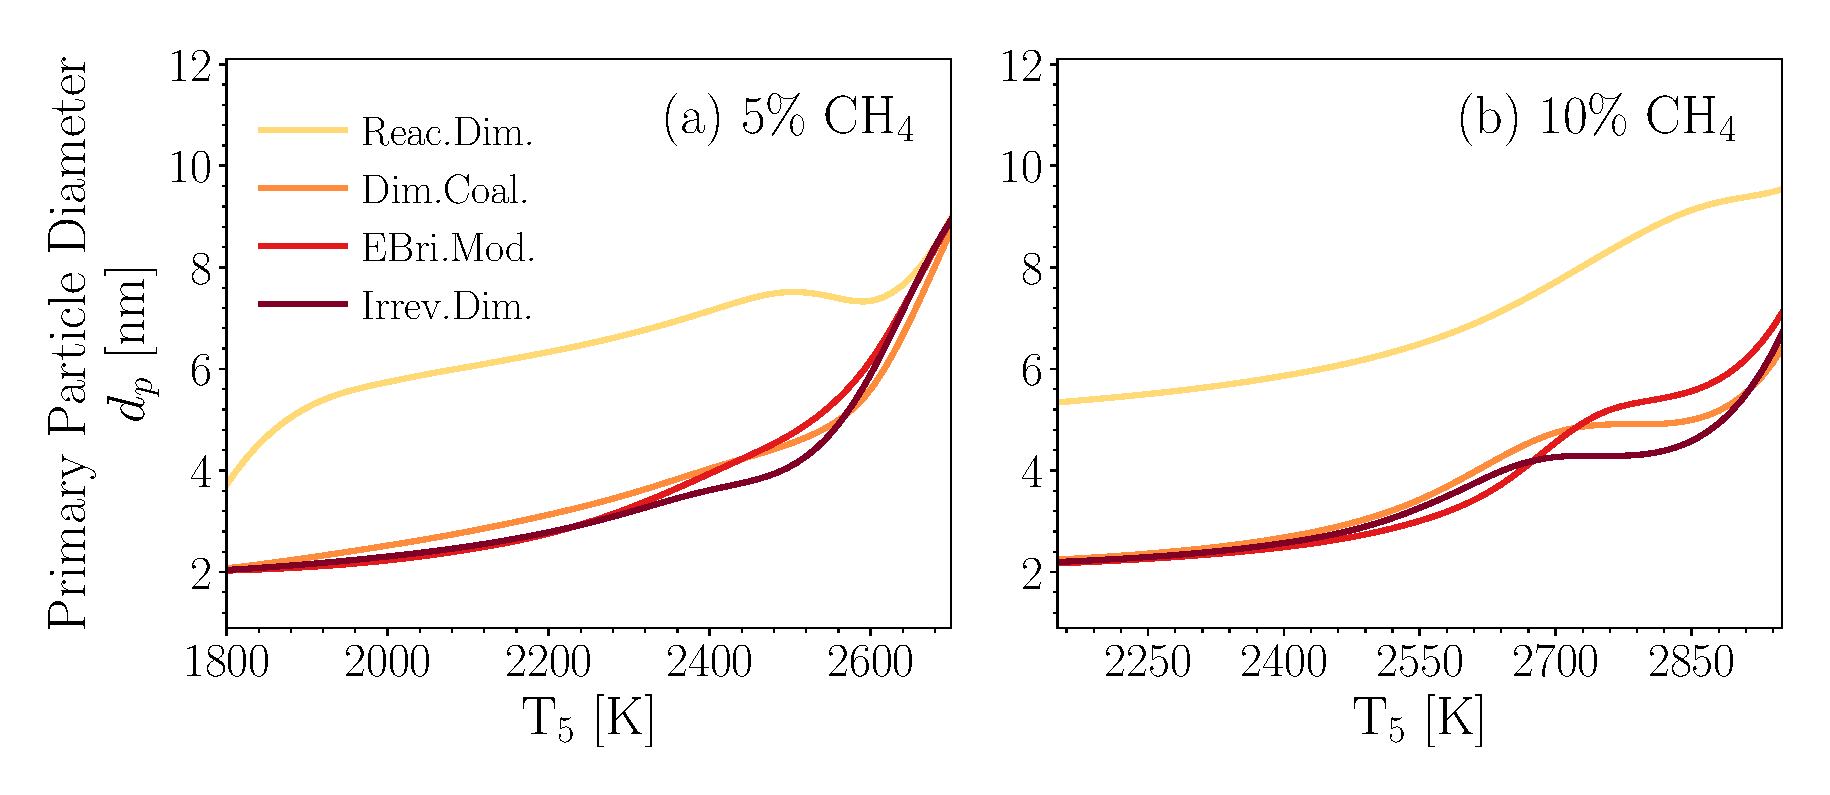
\includegraphics[width=0.8\textwidth]{Figures/Results/Shocktube/Agafonov2016_cvr/d_p.pdf}
%	\caption{The temperature dependence of mean primary particle diameter, $d_p$ at t=1.5 ms for 5\% (a) and 10\%~$\mathrm{CH_4}$ (b) in Ar obtained using Caltech mechanism and different inception models calibrated to minimize the prediction with extinction measurements~\citep{agafonov2016unified}.}
%	\label{fig:shockagof_dp_cvr} 
%\end{figure}
%
%Figure\ref{fig:shockagof_dp} shows that $d_p$ increases with temperature up to 10 nm. For 5\% $\mathrm{CH_4}$, $d_p$ reaches the peak around 2800 K and drops quickly to 2 nm which is the minimum allowed diameter in the model. Reactive Dimerization results in overall larger primary particle diameters, but the behavior of the rest of inception models are similar.
%
%\begin{figure}[H]
%	\centering
%	\begin{tikzpicture}
%		\draw (0, 0) node[inner sep=0] 	{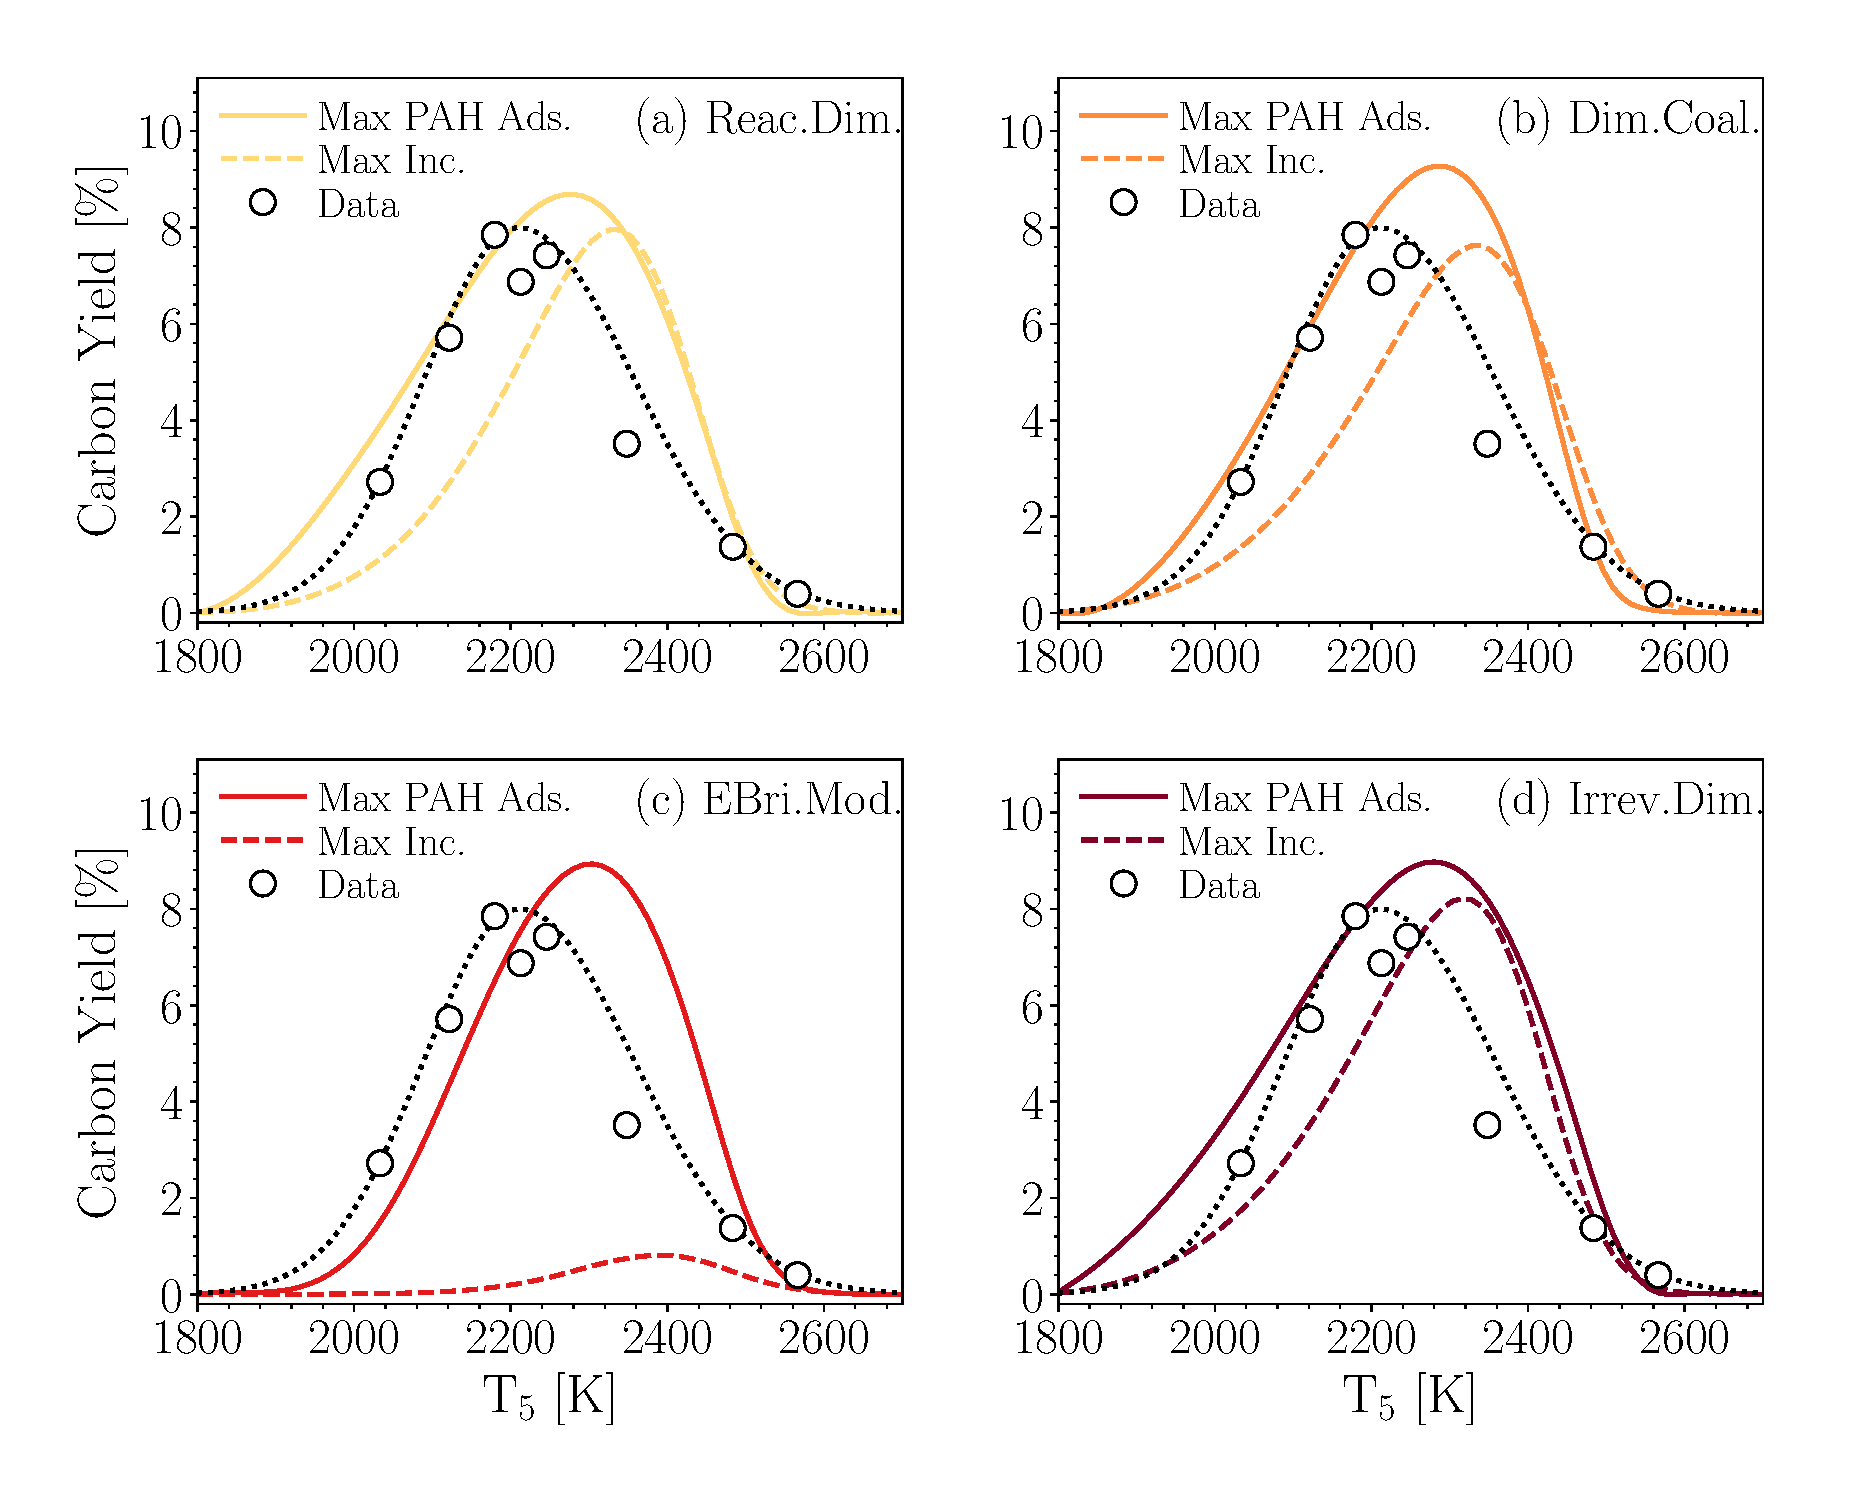
\includegraphics[width=0.8\textwidth]{Figures/Results/Shocktube/Agafonov2016_cvr/carbon_yield_maxincads.pdf}};
%		\draw (-3.18, -0.9) node {\scriptsize{\cite{agafonov2016unified}}};
%		\draw (2.46, -0.9) node {\scriptsize{\cite{agafonov2016unified}}};
%		\draw (-3.18, 3.55) node {\scriptsize{\cite{agafonov2016unified}}};
%		\draw (2.46, 3.55) node {\scriptsize{\cite{agafonov2016unified}}};
%	\end{tikzpicture}
%	\caption{The comparison of soot carbon yield at t=1.5 ms when maximum inception and PAH adsorption were applied to minimized the prediction  error compared to measurements~\citep{agafonov2016unified} for 5\% (a) and 10\%~$\mathrm{CH_4}$ (b) in Ar obtained using Caltech mechanism and different inception models.}
%	\label{fig:shockagof_yield_maxincads_cvr} 
%\end{figure}
%
%\begin{figure}[H]
%	\centering
%	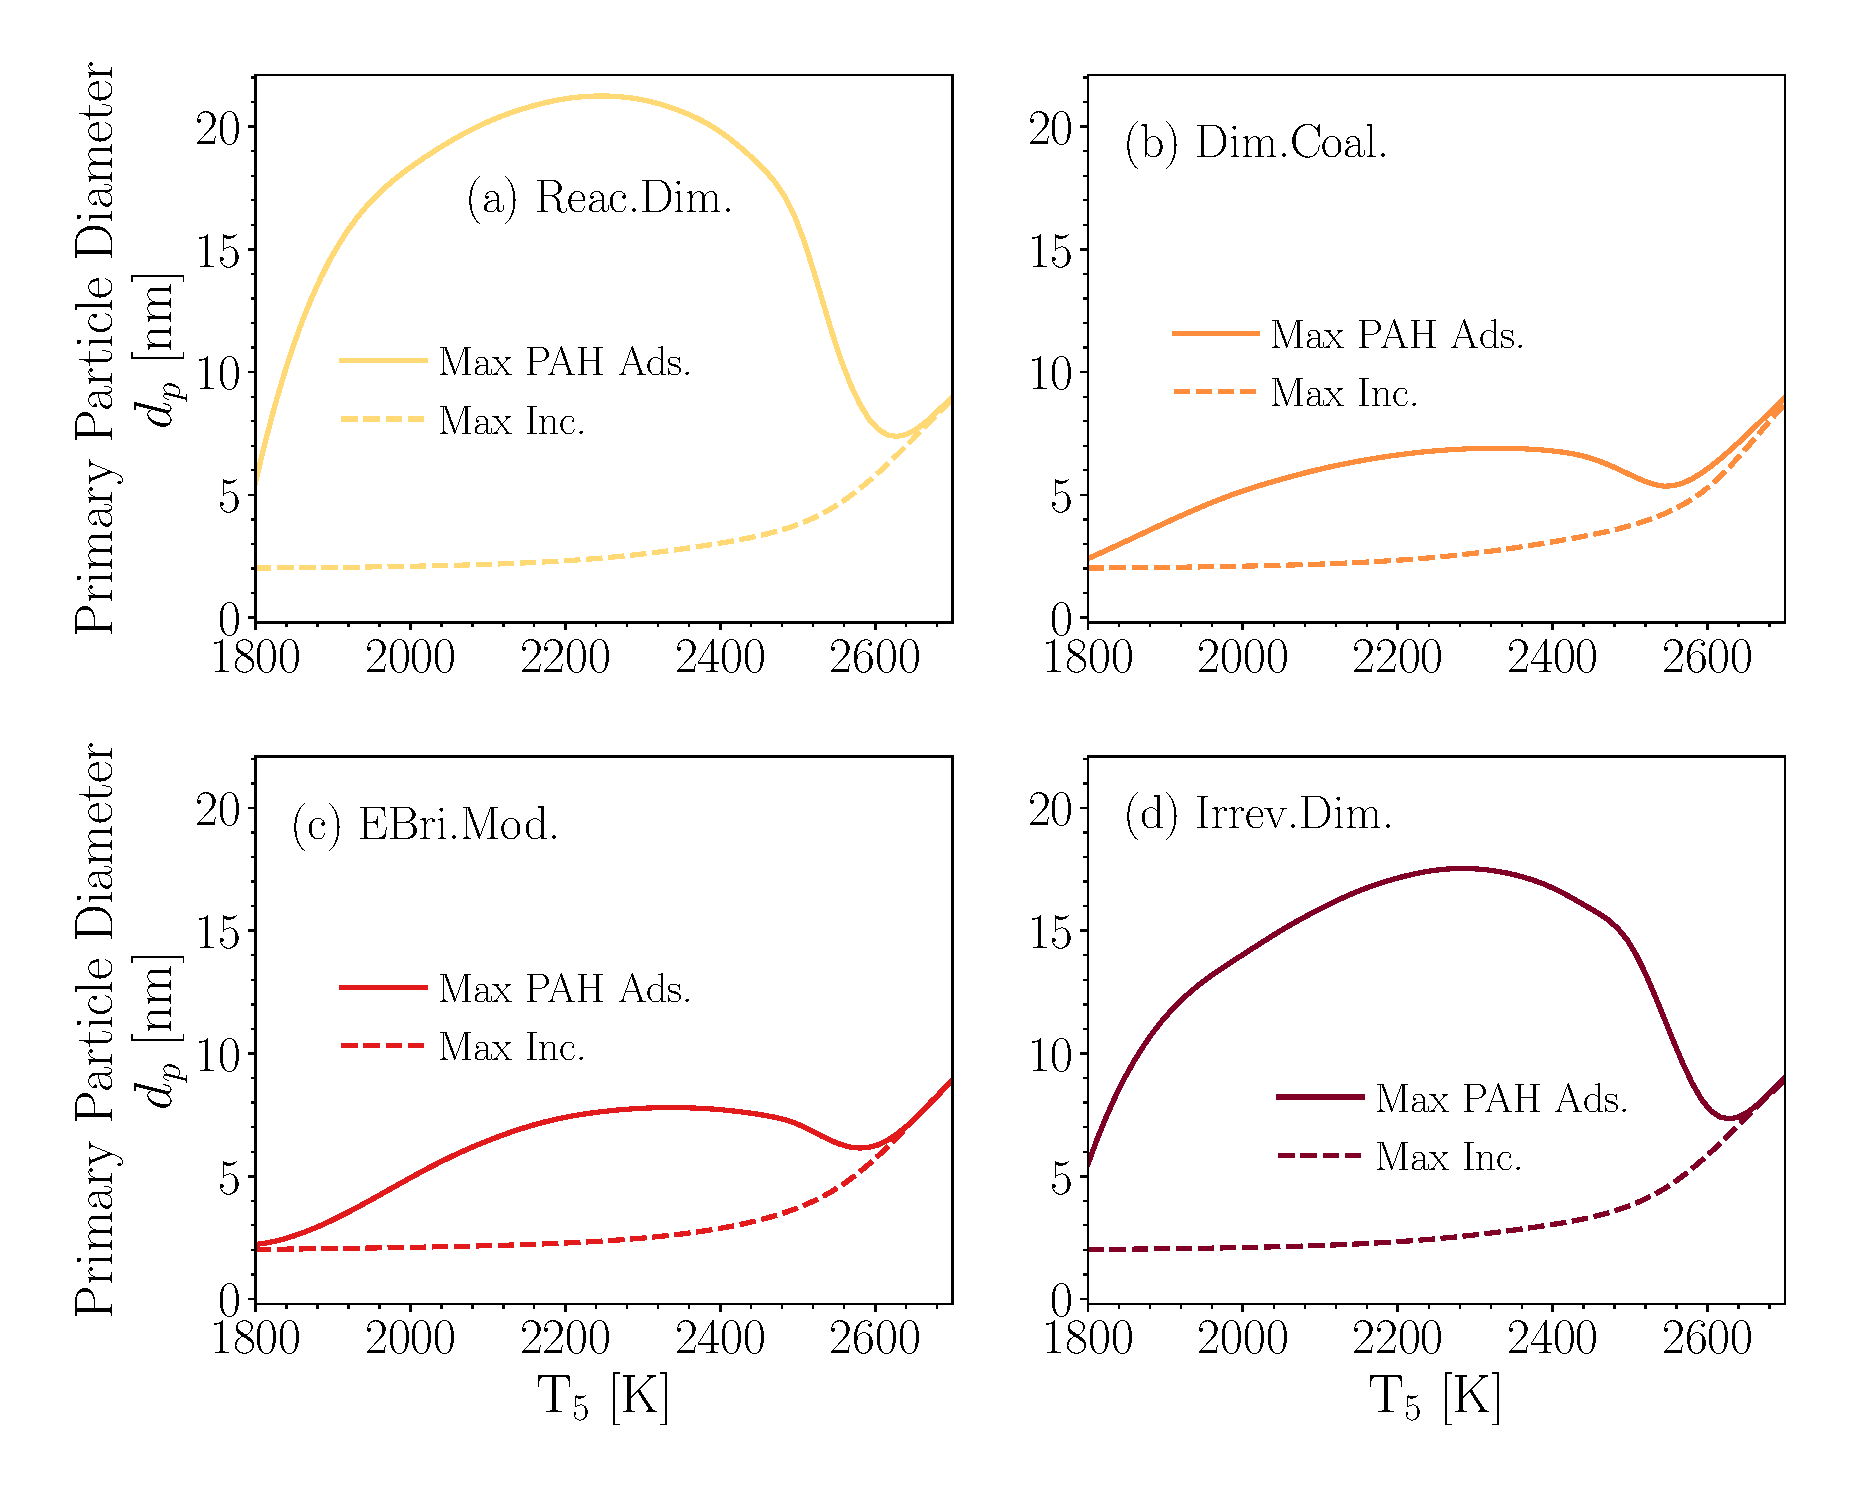
\includegraphics[width=0.8\textwidth]{Figures/Results/Shocktube/Agafonov2016_cvr/d_p_maxincads.pdf}
%	\caption{The comparison of mean primary particle, $d_p$ at t=1.5 ms when maximum inception and PAH adsorption were applied to minimized the prediction  error compared to measurements~\citep{agafonov2016unified} for 5\% (a) and 10\%~$\mathrm{CH_4}$ (b) in Ar obtained using Caltech mechanism and different inception models.}
%	\label{fig:shockagof_dp_maxincads_cvr} 
%\end{figure}